\documentclass{article}
\usepackage{amsmath, amssymb}
\usepackage[dvipsnames]{xcolor}
\usepackage{wasysym}
\usepackage{graphicx}

\DeclareMathAlphabet{\mymathbb}{U}{BOONDOX-ds}{m}{n}

\begin{document}
  \begin{center} \Large
    MA-652 Advanced Calculus\\
    Homework 2, Jan. 13 \\
    Adam Frank
  \end{center}

  \vspace{1cm}

  {\Large \color{Sepia} Problem 1. Rudin page 114 problem 7. Suppose $f'(x),g'(x)$ exist, $g'(x)\ne 0$, and $f(x)=g(x)=0$.  Prove that

  \begin{align*}
    \lim_{t\to x}\frac{f(t)}{g(t)} = \frac{f'(x)}{g'(x)}
  \end{align*} }

  \vspace{1cm}

  \begin{align*}
    \lim_{t\to x}\frac{f(t)}{g(t)} = \lim_{t\to x}\frac{(f(t)-f(x))/(t-x)}{(g(t)-g(x))/(t-x)} = \frac{\lim_{t\to x}(f(t)-f(x))/(t-x)}{\lim_{t\to x}(g(t)-g(x))/(t-x)} = \frac{f'(x)}{g'(x)}
  \end{align*}

  Where the second equality is due to the fact that $g'(x)\ne 0$.

  \pagebreak

  {\Large \color{Sepia} Problem 2. Rudin page 114 problem 8. Suppose $f'$ is continuous on $[a,b]$ and $\varepsilon>0$.  Prove that there exists a $\delta>0$ such that $\left|\frac{f(t)-f(x)}{t-x}-f'(x)\right|<\varepsilon$ whenever $0<|t-x|<\delta$, for $a\leq x\leq b$, $a\leq t\leq b$.  Does this hold for vector-valued functions?}

  \vspace{1cm}

  Since $f'$ is continuous on a compact set it is uniformly continuous.  Hence

  \begin{align*}
    |f'(t)-f'(x)|<\varepsilon
  \end{align*}

  for some $\delta$ and all $|t-x|<\delta$.  By the mean value theorem there is some $c$ between $t$ and $x$ such that

  \begin{align*}
    f'(c) = \frac{f(t)-f(x)}{t-x}
  \end{align*}

  Now since $c$ is between $t$ and $x$ we must have $|c-x|<|t-x|<\delta$ and hence by our initial assumption,

  \begin{align*}
    \left|\frac{f(t)-f(x)}{t-x}-f'(x)\right| = |f'(c)-f'(x)| < \varepsilon
  \end{align*}

  \vspace{1cm}

  This also holds for vector-valued functions.  Suppose $\vec f$ is a vector-valued function $\vec f: [a,b]\to \mathbb R^n$.  Say the components are $f_i$ for $i=1,\dots,n$.  For any $\varepsilon$ we can choose $\delta_1, \delta_2, ...,\delta_n$ such that for each $i=1,2,...,n$ we have $\left|\frac{f_i(t)-f_i(x)}{t-x} - f_i'(x)\right|<\varepsilon/n$ whenever $|t-x|<\delta_i$.   Then set $\delta = \min\{\delta_1, \dots, \delta_n\}$.  If $|t-x|<\delta$ then

  \begin{align*}
    \left|\frac{\vec f(t)-\vec f (x)}{t-x}-\vec f'(x)\right| \leq \sum\left|\frac{f_i(t)-f_i(x)}{t-x} - f_i'(x)\right| < n(\varepsilon/n) = \varepsilon
  \end{align*}

  \pagebreak

  {\Large \color{Sepia} Problem 3. Rudin page 115 problem 9. Let $f$ be a continuous real function on $\mathbb R$, of which it is known that $f'(x)$ exists for all $x\ne 0$ and that $f'(x)\to 3$ as $x\to 0$.  Does it follow that $f'(0)$ exists?}

  \vspace{1cm}

  Yes.  {\it Proof:}  By L'Hospital's Rule, since the derivative has the form 0/0, we have

  \begin{align*}
    f'(0) = \lim_{x\to 0}\frac{f(x)-f(0)}{x-0} = \lim_{x\to 0}\frac{f'(x)}{1}=3
  \end{align*}

  \pagebreak

  {\Large \color{Sepia} Problem 4. Rudin page 115 problem 11. Suppose $f$ is defined in a neighborhood of $x$, and suppose $f''(x)$ exists.  Show that

  \begin{align*}
    \lim_{h\to 0} \frac{f(x+h)+f(x-h)-2f(x)}{h^2} = f''(x)
  \end{align*}

  Show by an example that the limit may exist even if $f''(x)$ does not. {\it Hint: Use Theorem 5.13.}}

  \vspace{1cm}

  Note that as $h\to 0$ both $h^2\to 0$ and also $f(x+h)-f(x-h)-2f(x)\to 0$ since $f''(x)$ exists and therefore $f'(x)$ exist, and so $f$ is continuous at $x$.  So by theorem 5.13,

  \begin{align*}
    \lim_{h\to 0}\frac{f(x+h)+f(x-h)-2f(x)}{h^2} &= \lim_{h\to 0}\frac{f'(x+h)-f'(x-h)}{2h} \\\\
    &= \frac 1 2 \lim_{h\to 0} \frac{f'(x+h)-f'(x)+f'(x)-f(x-h)}{h}
  \end{align*}

  and this again is of the form 0/0, and so is equal to

  \begin{align*}
    \frac 1 2 \lim_{h\to 0}\frac{f''(x+h)+f''(x-h)}{1} = \frac 1 2 (2f''(x)) = f''(x)
  \end{align*}

  where this limit exists by the given assumptions.

  \vspace{1cm}

  To see an example where the limit exists even when $f''$ does not we can take

  \begin{align*}
    g(x) = \begin{cases}
      -x^2 & \text{ if } x < 0\\
      x^2 & \text{ if } x\geq 0
    \end{cases}
  \end{align*}

  Then

  \begin{align*}
    g'(x) = \begin{cases}
      -2x & \text{ if } x < 0\\
      2x & \text{ if } x\geq 0
    \end{cases}
  \end{align*}

  which we can see by finding the derivative on three regions, $(-\infty, 0), \{0\},$ and $(0,\infty)$.  But the derivative of the above does not exist at 0, since the left-handed derivative is $-2$, and the right-handed derivative is 2.

  \pagebreak

  {\Large \color{Sepia} Problem 5. Rudin page 115 problem 12. If $f(x)=|x^3|$, compute $f'(x), f''(x)$ for all real $x$, and show that $f^{(3)}(0)$ does not exist.}

  \vspace{1cm}

  If $x\ne 0$ then we can compute $f'(x)$ on some interval $|t-x|<x$.  If $x>0$ then $f'(x)=(x^3)'=3x^2$ and if $x<0$ then $f'(x)=(-x^3)=-3x^2$.  At $x=0$

  \begin{align*}
    \lim_{t\to 0^+}\frac{f(t)-f(0)}{t-0} = \lim_{t\to 0^+}\frac{t^3}{t} = 0
  \end{align*}

  because we know this is the limit from the right for the difference quotient of $x^3$.  Likewise

  \begin{align*}
    \lim_{t\to 0^-}\frac{f(t)-f(0)}{t-0} = \lim_{t\to 0^-}\frac{-t^3}{t}=0
  \end{align*}

  Since the left and right limits are equal, this is the limit.

  By the same process we can compute $f''$ where $x>0$, in which case this is just $6x$, and where $x<0$ this is $-6x$.  And where $x=0$ we can again take right and left limits and confirm that both are 0.

  For $f''$ we can again show that when $x<0$ we have $f''(x)=-6$ and when $x>0$ we have $f''(x)=6$.  However,

  \begin{align*}
    \lim_{t\to 0^+}\frac{f'(t)-f'(0)}{t-0}=\lim_{t\to 0^+}\frac{6t}{t} = 6\\\\
    \lim_{t\to 0^-}\frac{f'(t)-f'(0)}{t-0}=\lim_{t\to 0^+}\frac{-6t}{t}=-6\
  \end{align*}

  Since these limits are unequal the derivative does not exist at $x=0$.

  \pagebreak

  {\Large \color{Sepia} Problem 6. Let $a\in \mathbb R$ and $f:(a,\infty)\to \mathbb R$ be twice differentiable. (a) Use Taylor's Theorem to show that $f'(x)=\frac{1}{2h}[f(x+2h)-f(x)]-hf''(\xi)$ for some $\xi \in (x,x+2h)$.}

  \vspace{1cm}

  Using the second Taylor polynomial on the interval $[x,x+2h]$, we set $\alpha=x, \beta=x+2h$.  Then there exists a $\xi\in(x,x+2h)$ such that

  \begin{align*}
    f(x+2h) = \\
    &f^{(0)}(x)(x+2h-x)^0+f^{(1)}(x)(x+2h-x)^1+\frac{f^{(2)}(\xi)}{2!}(x+2h-x)^2
  \end{align*}

  therefore

  \begin{align*}
    f(x+2h)&=f(x)+f'(x)(2h) + \frac{f''(\xi)}{2}(2h)^2 \quad \Rightarrow \\\\
    f'(x) &= \frac{1}{2h}[f(x+2h)-f(x)]-f''(\xi)h
  \end{align*}

  \vspace{1cm}

  {\Large \color{Sepia} (b) Use the result from part (a) to show that if $M_0,M_1,M_2$ are the LUBs of $|f(x)|,|f'(x)|,$ and $|f''(x)|$ respectively on $(a,\infty)$, then $|f'(x)|\leq hM_2+\frac{M_0}{h}$.}

  \vspace{1cm}

  \begin{align*}
    |f'(x)| &\leq \frac{1}{2h}  |f(x+2h)-f(x)|+ |f''(\xi)|h \\\\
    &\leq \frac{1}{2h}(|f(x+2h)|+|f(x)|)+M_2h \\\\
    &\leq \frac{1}{2h}(2M_0)+M_2h \\\\
    &= hM_2+\frac{M_0}{h}
  \end{align*}

  \vspace{1cm}

  {\Large \color{Sepia} (c) Use part (b) to show $M_1^2\leq 4M_0M_2$.}

  \vspace{1cm}

  From the above $M_1\leq hM_2+\frac{M_0}{h}$ and so

  \begin{align*}
    M_1^2\leq h^2M_2^2+2M_0M_2+\frac{M_0^2}{h^2}
  \end{align*}

  It then suffices to prove that $h^2M_2^2+\frac{M_0^2}{h^2}\leq 2M_0M_2$.  We attempt to minimize $g(h)=h^2M_2^2+\frac{M_0^2}{h^2}$.

  \begin{align*}
    g'(h) = 2hM_2^2-2\left(\frac{M_0^2}{h^3}\right) = 0 \quad \Rightarrow \\\\
    h^4M_2^2-M_0^2 = 0 \quad \Rightarrow \\\\
    h^4 = (M_0/M_1)^2 \quad \Rightarrow \\\\
    h = \sqrt{M_0/M_1}
  \end{align*}

  And this is a minimum because the second derivative is positive everywhere:

  \begin{align*}
    g''(h) = 2M_2^2+6M_0^2/h^4
  \end{align*}

  Hence we have that $g(\sqrt{M_0/M_1})\leq g(h)$ for each $h$ and hence

  \begin{align*}
    (\sqrt{M_0/M_1})^2M_2^2 + \frac{M_0^2}{(\sqrt{M_0/M_1})^2} = 2M_0M_1 \leq h^2M_2^2+\frac{M_0^2}{h^2}
  \end{align*}

  Hence we have shown $M_1^2\leq 4M_0M_2$.

  \pagebreak

  {\Large \color{Sepia} Problem 7. Rudin part 116 problem 16. Suppose $f$ is twice differentiable on $(0,\infty)$, $f''$ is bounded on $(0,\infty)$, and $f(x)\to 0$ as $x\to \infty$.  Prove that $f'(x)\to 0$ as $x\to \infty$.  {\it Hint:} Let $a\to \infty$ in exercise 15.}

  \vspace{1cm}

  Define

  \begin{align*}
    M_0(a) &= \sup\{|f(x)|: \ a < x < \infty\} \\
    M_1(a) &= \sup\{|f'(x)|: \ a < x < \infty\} \\
    M_2(a) &= \sup\{|f''(x)|: \ a < x < \infty\}
  \end{align*}

  so that the earlier exercise entails that for each $a>0$ we have $[M_1(a)]^2 \leq 4M_0(a)M_2(a)$.  Moreover since $f(x)\to 0$ as $x\to \infty$, hence $M_0(a)\to 0$ as $a\to \infty$.  And since there is some bound $A\in [0,\infty)$ such that $|f''(x)|\leq A$ then $M_2(a)\leq A$ for each $a$.  Hence as $a\to \infty$ we have $4M_0M_2\to 0$ and thus $M_1^2(a)\to 0$.  This then implies that $M_1(a)\to 0$ as $a\to \infty$, and therefore as $a\to \infty$ we have $x\to \infty$ and $f'(x)\to 0$.

  \pagebreak

  {\Large \color{Sepia} Problem 8. Rudin part 116 problem 25. Suppose $f$ is twice differentiable on $[a,b], f(a)<0, f(b)>0, f'(x)\geq \delta>0$, and $0\leq f''(x)\leq M$ for all $x\in[a,b]$.  Let $\xi$ be the unique point in $(a,b)$ at which $f(\xi)=0.$  Complete the details in the following outline of Newton's method for computing $\xi$.

  (a) Choose $x_1\in (\xi,b)$ and define $\{x_n\}$ by

  \begin{align*}
    x_{n+1}=x_n-\frac{f(x_n)}{f'(x_n)}
  \end{align*}

  Interpret this geometrically in terms of the tangent to the graph of $f$.}

  \vspace{1cm}

  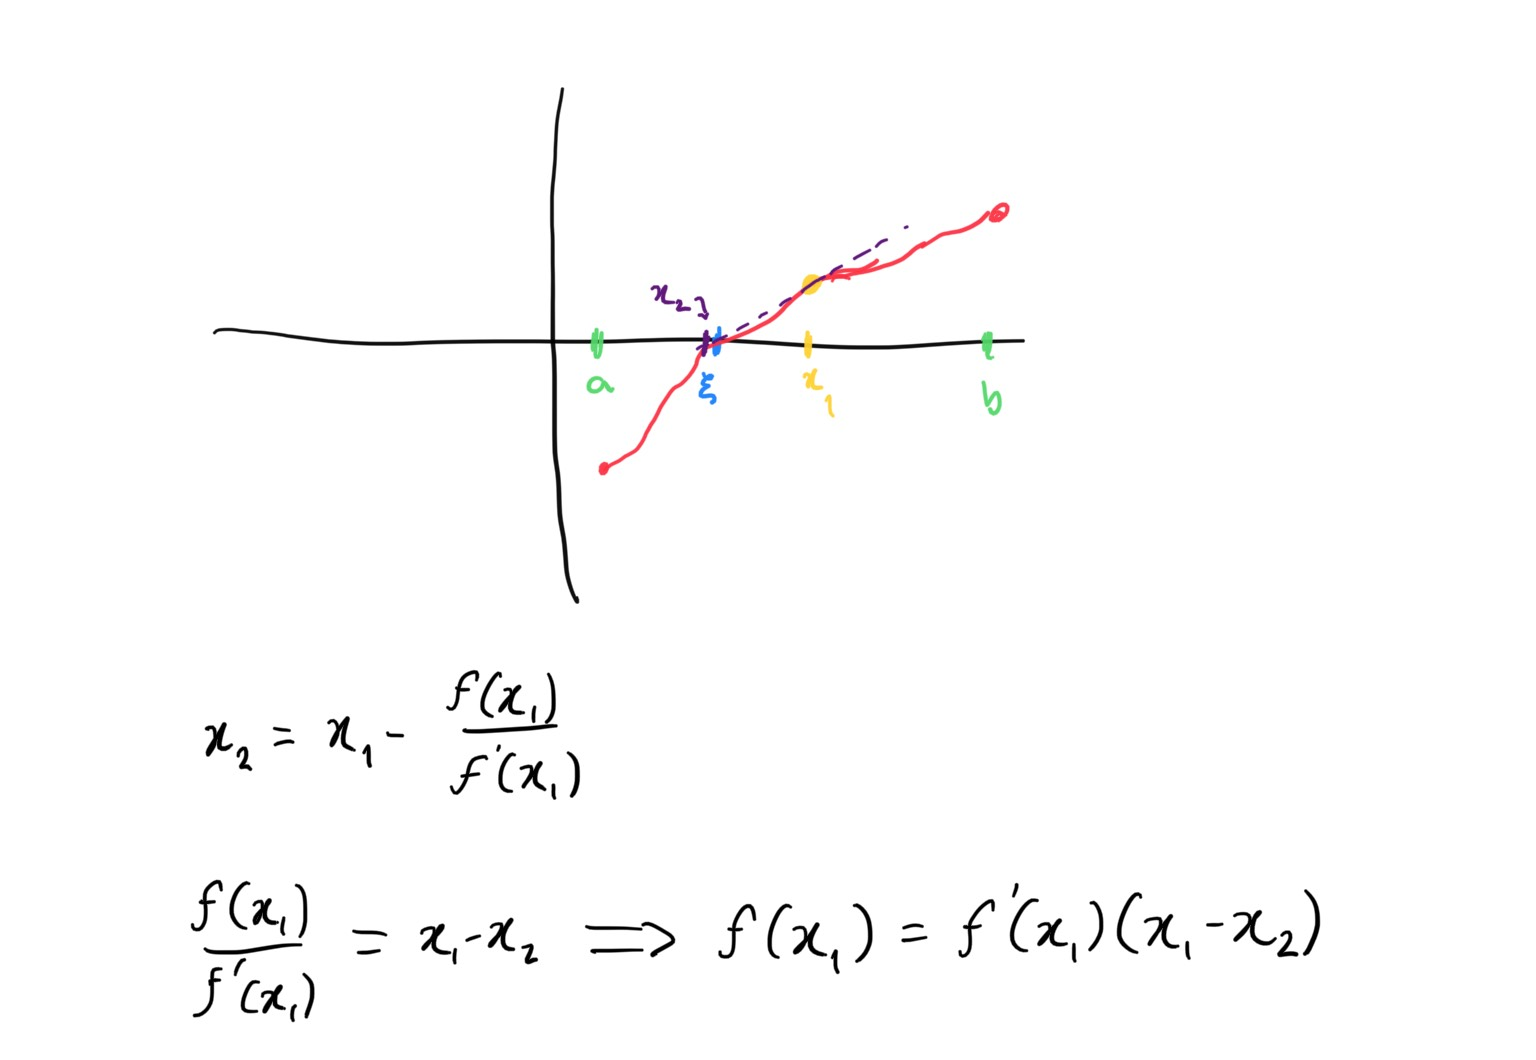
\includegraphics[scale=.2]{drawing.jpg}

  Of course $x_1$ is arbitrary (although a point to the right of a zero, for an increasing function).  $f(x_1)$ is the "height" of the function at $x_1$ and $f'(x_1)$ the slope of the linearization at this point.  $x_2$ is then the point where the linearization intersects the $x$-axis.  Hopefully it is therefore a good approximation of the zero of $f$.

  And in the same way, each next $x_{n+1}$ is a better approximation taken from the ``starting point" of $x_n$.

  \vspace{1cm}

  {\Large \color{Sepia} (b) Prove that $x_{n+1}<x_n$ and that $\lim_{n\to \infty}x_n=\xi$.}

  \vspace{1cm}

  We begin by proving by induction that $x_n \geq \xi$ for all $n\in\mathbb Z^+$.  First note that if $x_n=\xi$ for any $\xi$ then $x_{n+1}=x_n-\frac{f(x_n)}{f'(x_n)}=\xi - \frac{f(\xi)}{f'(x_n)} = \xi$.  And moreover for each $m\in\mathbb Z^+$ it follows that $x_{n+m}=\xi$ and therefore trivially $\displaystyle \lim_{n\to\infty}x_n=\xi$.  So for the remaining cases, we assume that $x_n\ne \xi$ for any $n\in\mathbb Z^+$.  Also, before beginning the proof, we remark that $f'$ is monotonically increasing because $f''$ is non-negative on this interval.

  The base case for the induction is immediate since $x_1\in(\xi,b)$.  For the inductive case suppose the claim holds up to $x_n$ and we will show that it also holds for $x_{n+1}$.  If we apply the mean value theorem to $f$ on the interval $(\xi, x_n)$ then there is some $c\in (\xi, x_n)$ such that

  \begin{align*}
    f'(c)=\frac{f(x_n)-f(\xi)}{x_n-\xi} = \frac{f(x_n)}{x_n-\xi}
  \end{align*}

  Now since $f'$ is increasing $f'(c)=\frac{f(x_n)}{x_n-\xi}\leq f'(x_n)$.  Now we can infer

  \begin{align*}
    x_{n+1}&=x_n-\frac{f(x_n)}{f'(x_n)} = x_n-\frac{f(x_n)}{f'(x_n)}\cdot \frac{x_n-\xi}{x_n-\xi} \\\\
    &\geq x_n-\frac{f'(x_n)(x_n-\xi)}{f'(x_n)}=x_n-(x_n-\xi)=\xi
  \end{align*}

  Now that we have completed the induction, we proceed to show that $x_{n+1}<x_n$.  It suffices to show $x_n-x_{n+1}=\frac{f(x_n)}{f'(x_n)}\geq 0$.  Since we know that $f'(x)$ is positive for all $x$ in the interval, $f'(x_n)>0$.  And since $x_n>\xi$ and since $f$ is increasing, then $f(x_n)>f(\xi)=0$.  Hence $\frac{f(x_n)}{f'(x_n)}>0$ and so the sequence $x_n$ is increasing.

  We have now established that the sequence is increasing and bounded below, hence by the monotone convergence theorem its limit exists.  Call the limit $\ell = \displaystyle\lim_{n\to\infty}x_n$.  Then since $f'$ and $f''$ both exist throughout the interval, these are continuous.  Hence

  \begin{align*}
    \lim_{n\to\infty}x_{n+1}=\lim_{n\to\infty}\left(x_n-\frac{f(x_n)}{f'(x_n)}\right) \\\\
    \ell = \ell - \frac{\lim_{n\to \infty}f(x_n)}{\lim_{n\to\infty}f'(x_n)}=\ell-\frac{f(\ell)}{f'(\ell)} \quad \Rightarrow \\\\
    \frac{f(\ell)}{f'(\ell)}=0\quad \Rightarrow \\\\
    f(\ell)=0
  \end{align*}

  Since $f$ has a unique zero, then $\ell = \displaystyle\lim_{n\to\infty}x_n=\xi$.

  \vspace{1cm}

  {\Large \color{Sepia} (c) Use Taylor's theorem to show that $x_{n+1}-\xi = \frac{f''(t_n)}{2f'(x_n)}(x_n-\xi)^2$ for some $t_n\in(\xi,x_n)$.}

  \vspace{1cm}

  Using Taylor's Theorem on the interval, set $\alpha=x_n$ and set $\beta=\xi$, and $n=2$.  Then there exists a $t_n\in (\xi,x_n)$ such that

  \begin{align*}
    f(\xi)&=0=P(\xi)+\frac{f^{(2)}(t_n)}{2!}(\xi-x_n)^2 \\\\
    &=\frac{f^{(0)}(x_n)}{0!}(\xi-x_n)^0+\frac{f^{(1)}(x_n)}{1!}(\xi-x_n)^1+\frac{f^{(2)}(t_n)}{2!}(\xi-x_n)^2 \\\\
    &= f(x_n) f'(x_n)(\xi-x_n)+\frac{f''(t_n)}{2}(x_n-\xi)^2
  \end{align*}

  Therefore

  \begin{align*}
    \frac{f''(t_n)(x_n-\xi)^2}{2}&= -(f(x_n)-f'(x_n)(\xi-x_n)) \quad \Rightarrow \\\\
    &\frac{f''(t_n)(x_n-\xi)}{2f'(x_n)} = x_n-\frac{f(x_n)}{f'(x_n)}+\xi = x_{n+1}-\xi
  \end{align*}

  \vspace{1cm}

  {\Large \color{Sepia} (d) If $A=M/2\delta$ deduce that

  \begin{align*}
    0\leq x_2-\xi \leq \frac 1 A [A(x_1-\xi)]^{2^n}
  \end{align*}}

  \vspace{1cm}

  From part (b) we already have that $x_{n+1}\geq \xi$ and so $0\leq x_{n+1}-\xi$.  For $x_{n+1}-\xi\leq \frac 1 A[A(x_1-\xi)]^{2^n}$ The proof is by induction on $n$.  For the base case, $n=1$, we need to show

  \begin{align*}
    x_{2}-\xi \leq \frac 1 A [A(x_1-\xi)]^{2^1} = A(x_1-\xi)^2
  \end{align*}

  From the previous part we have for some $t_1\in(\xi,x_1)$

  \begin{align*}
    x_2-\xi = \frac{f''(t_1)(x_1-\xi)^2}{2f'(x_n)}(x_1-\xi)^2 \leq \frac{M}{2\delta}(x_1-\xi)^2=A(x_1-\xi)^2
  \end{align*}

  where the inequality follows because $f''(x)\leq M$ and $f'(x)>\delta$ For each $x$ in the interval.

  Now for the inductive case we assume this holds up to $n$ and show that it then holds for $n+1$.  In particular we assume

  \begin{align*}
    x_n-\xi \leq \frac 1 A[A(x_1-\xi)]^{2^n}
  \end{align*}

  and want to show

  \begin{align*}
    x_{n+1}-\xi\leq \frac 1 A[A(x_1-\xi)]^{2^{n+1}}
  \end{align*}

  From part (c) we again have that

  \begin{align*}
    x_{n+1}-\xi\leq \frac {f''(x_n)}{2f'(x_n)}(x_n-\xi)^2 \leq A\left[\frac 1 A(A[x_1-\xi])^{2^n}\right]^2 = \frac 1 A (A[x_1-\xi])^{2^{n+1}}
  \end{align*}

  where this second inequality follows from the inductive hypothesis.  The inductive case is now complete, and we can conclude that

  \begin{align*}
    x_{n}-\xi \leq \frac 1 A(A[x_1-\xi])^{2^n}
  \end{align*}

  \vspace{1cm}

  {\Large \color{Sepia} (e) Show that Newton's method amounts to finding a fixed point of the function $g$ defined by

  \begin{align*}
    g(x) = x-\frac{f(x)}{f'(x)}
  \end{align*}

  How does $g'(x)$ behave for $x$ near $\xi$?}

  \vspace{1cm}

  Using Newton's Method $x_1$ is always arbitrary.  But $x_2=g(x_1)$ and in general $x_{n+1}=g^n(x_1)$.  This function has a fixed point when

  \begin{align*}
    g(x)  = x = x-\frac{f(x)}{f'(x)} \quad \Rightarrow\\\\
    \frac{f(x)}{f'(x)}=0 \quad \Rightarrow \\\\
    f(x)=0
  \end{align*}

  so that the fixed point of $g$ is the zero of $f$, which is what this limit converges to.

  \vspace{1cm}

  Since $g'(x)=1-\frac{(f'(x))^2-f(x)f''(x)}{(f'(x))^2}$ we can first note that as $x\to \xi$ the term $f(x)f''(x)\to 0$ and hence $1-\frac{(f'(x))^2-f(x)f''(x)}{(f'(x))^2}\to 1-\frac{(f'(x))^2}{(f'(x))^2} = 0$.

  \vspace{1cm}

  {\Large \color{Sepia} (f) Put $f(x)=x^{1/3}$ on $(-\infty,\infty)$ and try Newton's method.  What happens?}

  \vspace{1cm}

  We know in advance that $\xi=0$ is the zero, so we choose $x_1\in(0,\infty)$ arbitrarily and set it to $x_1=1$.  And we compute that at all points in $(0,\infty)$ we have

  \begin{align*}
    g'(x)=\frac 1 3 x^{-2/3}
  \end{align*}

  Then

  \begin{align*}
    x_2=1-\frac{1^{1/3}}{\frac 1 3 1^{-2/3}} = 1-3=-2
  \end{align*}

  Already $x_2\not\in (0,\infty)$, so Newton's method fails.  Of course for this function, its first derivative does not exist throughout the interval, and its second derivative is unbounded, hence it fails the conditions in two ways.

  And moreover, if we want to continue applying Newton's Method we'll see that the values only grow in absolute value.  For instance,

  \begin{align*}
    x_3 = -2-\frac{f(-2)}{f'(-2)} = -2 -\frac{(-2)^{1/3}}{\frac 1 3 (-2)^{-2/3}} = 4
  \end{align*}

  As this pattern continues the absolute values $|x_n|$ approach infinity, and the sequence does not converge to the zero of the function, which we know to be 0.

  \pagebreak



































\end{document}
